% Niveau :      PC
% Discipline :  Méca
% Mots clés :   Van Der Pol

\begin{exercise}{Oscillateur Van Der Pol}{3}{Spé}
{Mécanique, Oscillateur harmonique, Pendule, Référentiel non galiléen}{lelay}

Il est possible en utilisant le montages montré sur l'image ci-dessous de faire en sorte que deux pendules se synchronisent : 

{\centering
    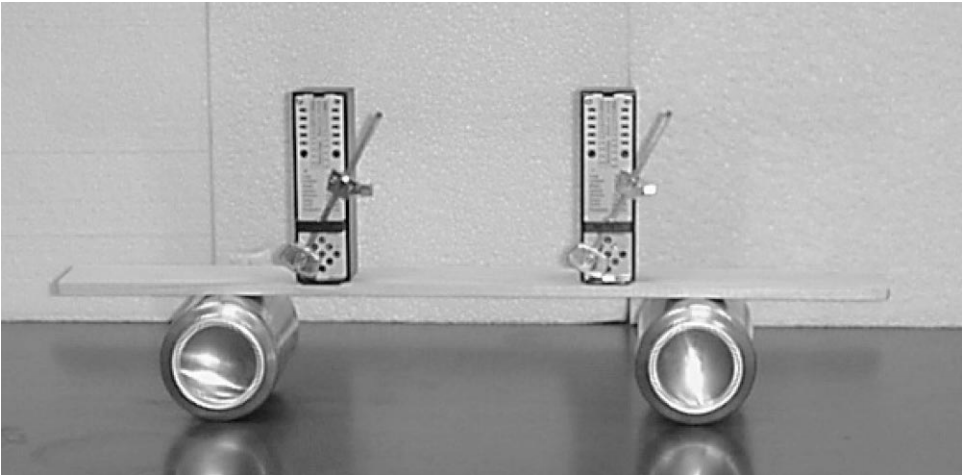
\includegraphics[scale=0.3]{meca/mecapoint/vanderpol.png}\par
}

Pour cet exercice, on considérera que les pendules sont auto-entretenus, que les canettes roulent sans glissement et que le mouvement d'un pendule auto-entretenu seul (sur une base fixe) est régi par l'équation dite de Van Der Pol : 
\begin{align*}
\frac{\dd^2 \theta}{\dd t^2} + \frac{g}L\sin\theta + \varepsilon\qty(\qty(\frac\theta{\theta_0})^2-1)\frac{\dd \theta}{\dd t}=0
\end{align*}

\begin{questions}
    \question Expliquer l'origine physique de chacun des termes de l'équation ci dessus.
    \question Justifier qu'un pendule obéissant à l'équation ci-dessus peut avoir un mouvement périodique d'amplitude constante. [Bonus : Le démontrer.]
	\question Établir l'équation du mouvement des deux pendules 
	\question Montrer qu'il peut y avoir synchronisation des pendules
\end{questions}
\end{exercise}